\section{BGP routing table}
\label{sec:bgp}


\subsection{Lengths of announced IP prefixes}

\begin{figure}[htbp]
	\centering
		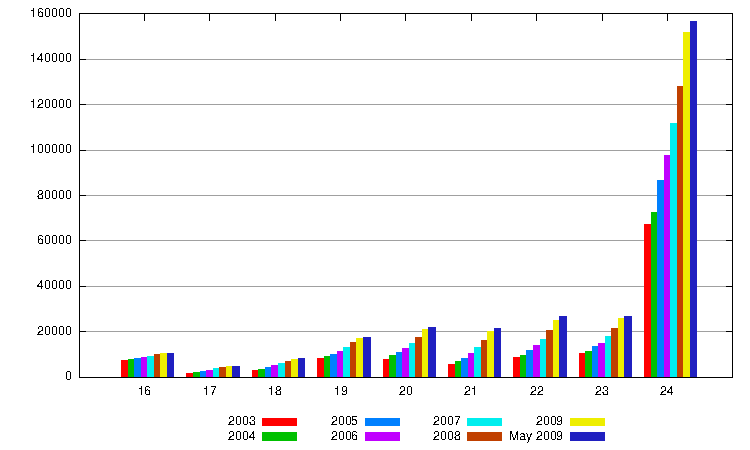
\includegraphics[width=\columnwidth]{02_prefixes/01_bgp_prefixes_zoom}
	\caption{Distribution of announced IP prefix lengths}
	\label{fig:bgp prefix distribution}
\end{figure}

\subsection{Age distribution of BGP entries}
Finally, eighth, we will provide a cumulative distribution function (CDF) of prefix ages, by which to draw conclusions about the stability of the routing table content. These will give information not so much about what is happening, but who is involved and for how long.
	
\begin{figure}[htbp]
	\centering
		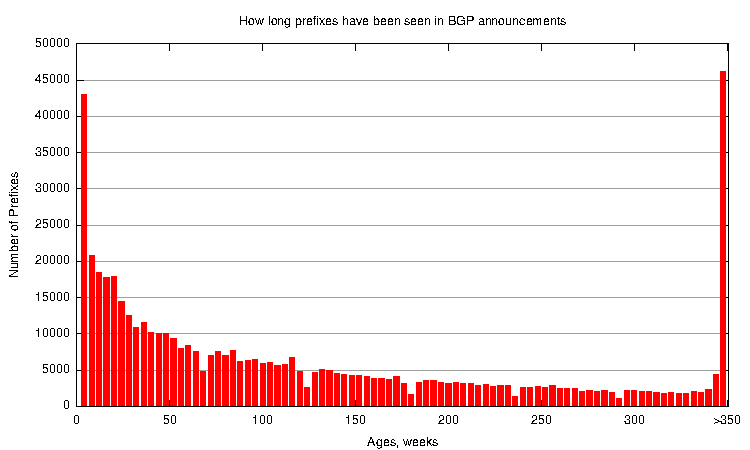
\includegraphics[width=\columnwidth]{08_ages/ages-4}
	\caption{Distribution of durations prefixes were visible in BGP announcements}
	\label{fig:bgp ages}
\end{figure}
	
\subsection{BGP announcements by geographical region}
One other direction of our BGP routing system study deals with characteristics of the allocations and announcements themselves.  These are in the areas of geography and age.  Some of the new areas we will examine to monitor where allocation activity is happening, and for how long a time on average.  Thus, seventh, we will give a year-on-year comparison of prefix allocations and prefix announcements by major countries, including Russia, Japan, major countries of Asia, and broad regions such as the European Union, North America, and Africa.

\begin{figure*}[p]
\centering

%%%%%%%%%%%%%%%%%%%%%%%%%%%%%%%%%%%%%%%%%%%%%%%%%%%%%%%%%%%%%%%%%%
%% BGP counts
%%%%%%%%%%%%%%%%%%%%%%%%%%%%%%%%%%%%%%%%%%%%%%%%%%%%%%%%%%%%%%%%%%
\begin{minipage}[b]{0.48\textwidth}
% \begin{figure}[p]
	\centering
		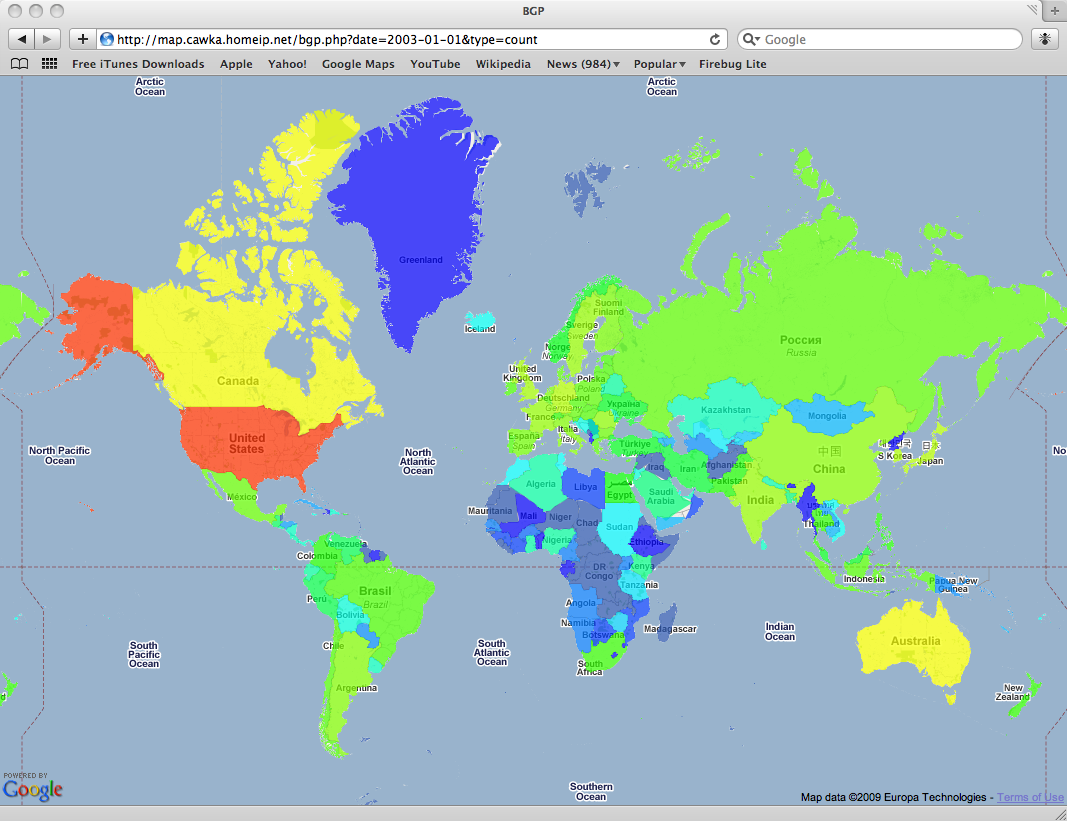
\includegraphics[trim=0 17px 0px 76px,clip=true,width=\columnwidth]{00_maps/bgp_count_2003}%
		\hspace{-0.98\columnwidth}%
		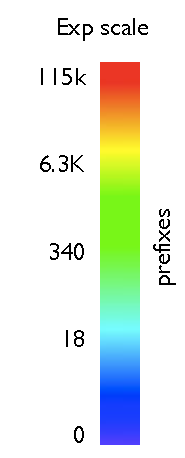
\includegraphics[width=1cm]{scale_bgp_count}\hspace{-1cm}%
		\hspace{0.98\columnwidth}
	\caption{Geographical distribution of number of announced prefixes on \textbf{January 1, 2003}}
	\label{fig:bgp prefixes 2003}
% \end{figure}
\end{minipage}%
%
\quad
%
\begin{minipage}[b]{0.48\textwidth}
% \begin{figure}[p]
	\centering
		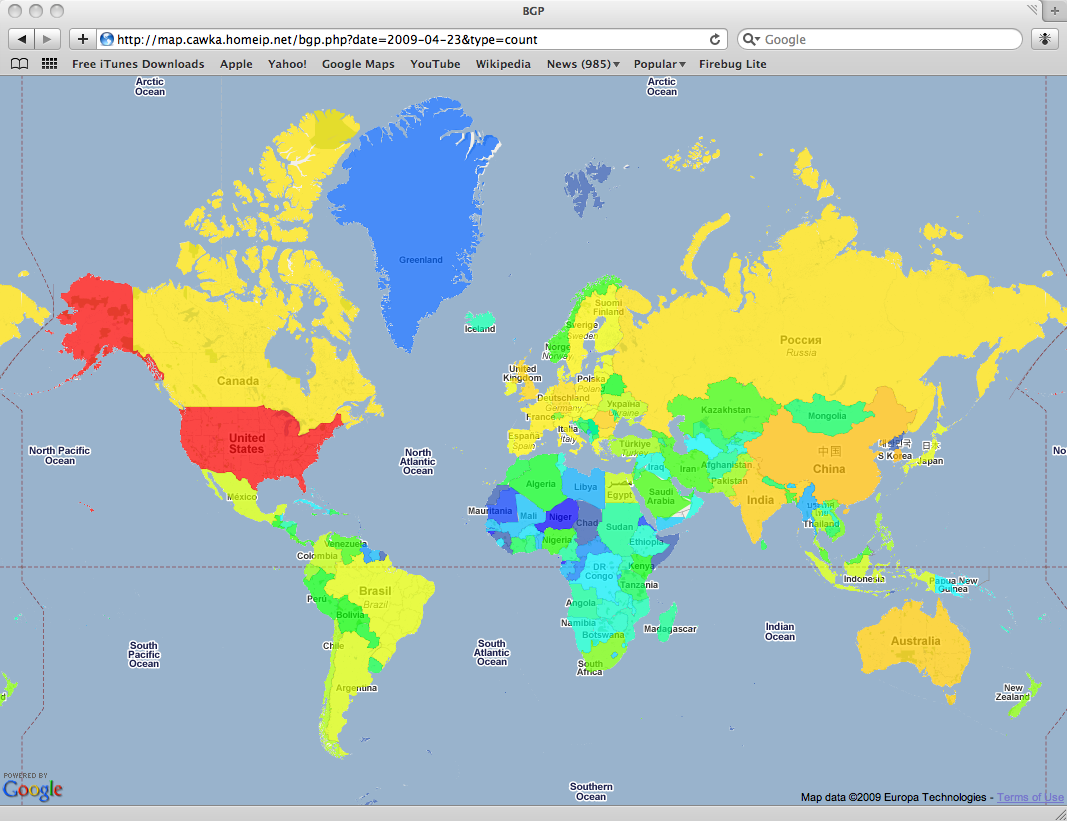
\includegraphics[trim=0 17px 0px 76px,clip=true,width=\columnwidth]{00_maps/bgp_count_2009_2}%
		\hspace{-0.98\columnwidth}%
		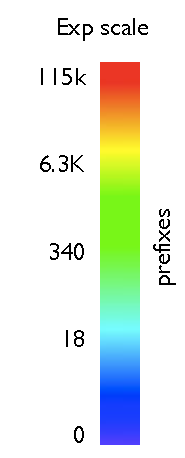
\includegraphics[width=1cm]{scale_bgp_count}\hspace{-1cm}%
		\hspace{0.98\columnwidth}
	\caption{Geographical distribution of number of announced prefixes on \textbf{April 23, 2009}}
	\label{fig:bgp prefixes 2009}
% \end{figure}
\end{minipage}

\vspace{0.5cm}

%%%%%%%%%%%%%%%%%%%%%%%%%%%%%%%%%%%%%%%%%%%%%%%%%%%%%%%%%%%%%%%%%%
%% BGP sizes
%%%%%%%%%%%%%%%%%%%%%%%%%%%%%%%%%%%%%%%%%%%%%%%%%%%%%%%%%%%%%%%%%%
\begin{minipage}[b]{0.48\textwidth}
% \begin{figure}[p]
	\centering
		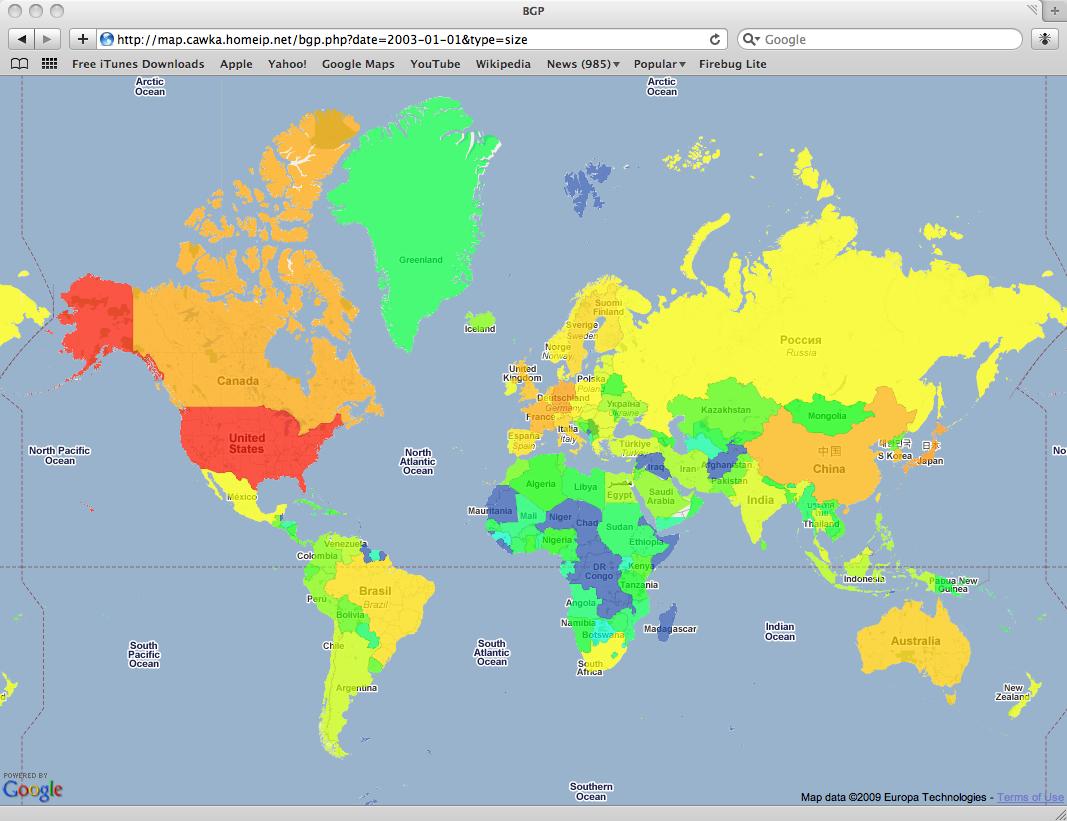
\includegraphics[trim=0 17px 0px 76px,clip=true,width=\columnwidth]{00_maps/bgp_size_2003}%
		\hspace{-0.98\columnwidth}%
		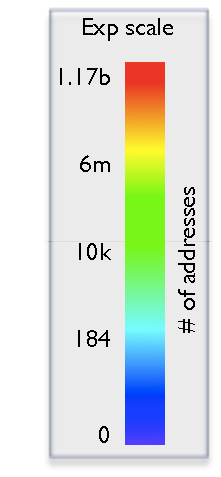
\includegraphics[width=1cm]{scale_bgp_size}\hspace{-1cm}%
		\hspace{0.98\columnwidth}
	\caption{Geographical distribution of announced IP space on \textbf{January 1, 2003}}
	\label{fig:bgp ip space 2003}
% \end{figure}
\end{minipage}%
%
\quad
%
\begin{minipage}[b]{0.48\textwidth}
% \begin{figure}[p]
	\centering
		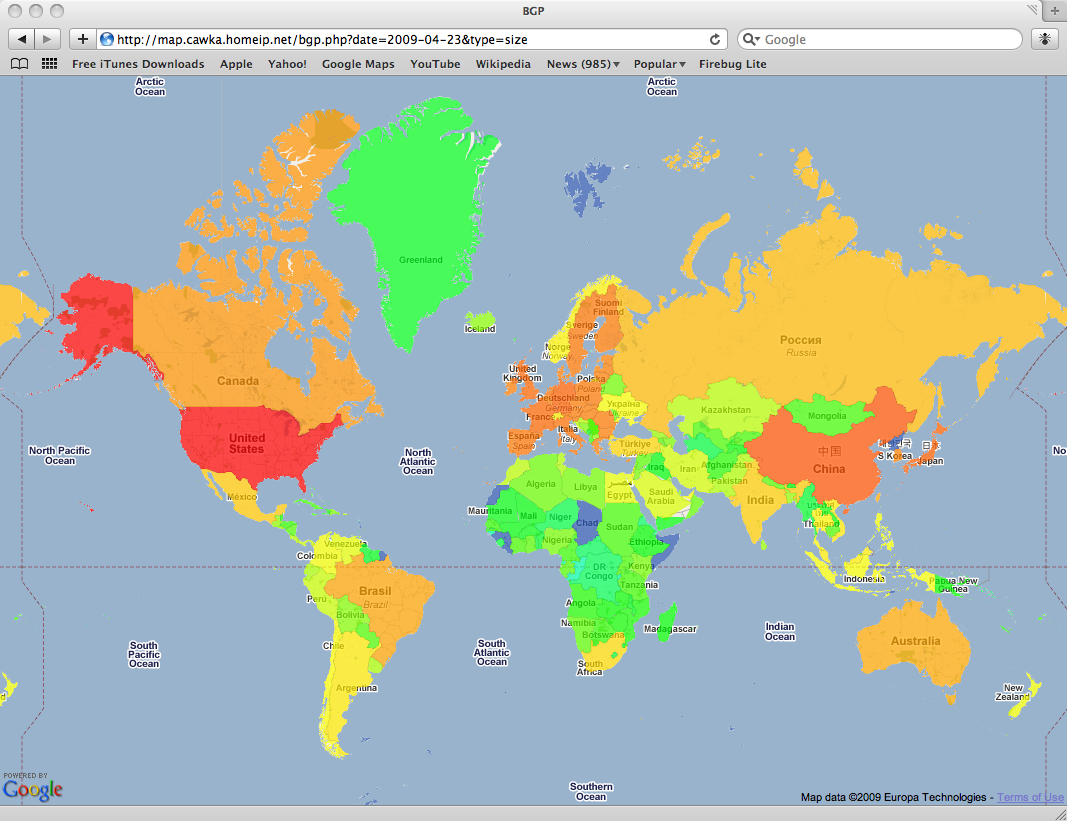
\includegraphics[trim=0 17px 0px 76px,clip=true,width=\columnwidth]{00_maps/bgp_size_2009_2}%
		\hspace{-0.98\columnwidth}%
		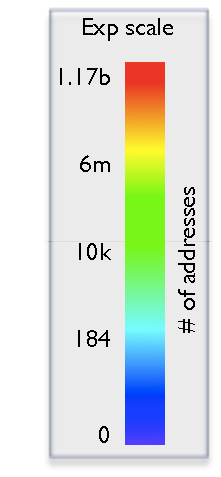
\includegraphics[width=1cm]{scale_bgp_size}\hspace{-1cm}%
		\hspace{0.98\columnwidth}
	\caption{Geographical distribution of announced IP space on \textbf{April 23, 2009}}
	\label{fig:bgp ip space 2009}
% \end{figure}
\end{minipage}

\vspace{0.5cm}

%%%%%%%%%%%%%%%%%%%%%%%%%%%%%%%%%%%%%%%%%%%%%%%%%%%%%%%%%%%%%%%%%%
%% Asia region
%%%%%%%%%%%%%%%%%%%%%%%%%%%%%%%%%%%%%%%%%%%%%%%%%%%%%%%%%%%%%%%%%%
\begin{minipage}[b]{0.48\textwidth}
% \begin{figure}[p]
	\centering
		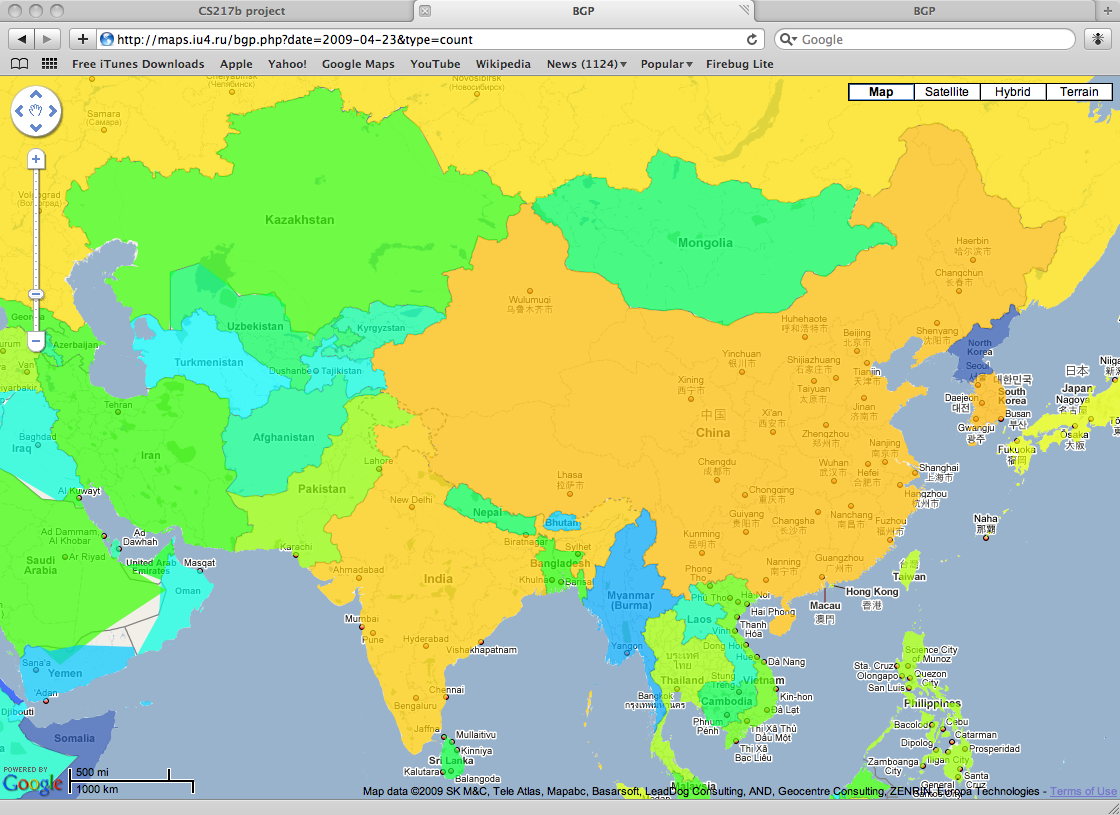
\includegraphics[trim=0 17px 0px 76px,clip=true,width=\columnwidth]{00_maps/asia_2009_prefixes}%
		\hspace{-0.98\columnwidth}%
		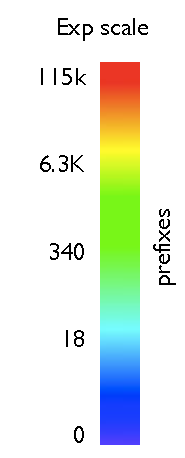
\includegraphics[width=1cm]{scale_bgp_count}\hspace{-1cm}%
		\hspace{0.98\columnwidth}
	\caption{Geographical distribution of number of announced prefixes in Asian region on \textbf{April 23, 2009}}
	\label{fig:bgp prefixes asia 2009}
% \end{figure}
\end{minipage}%
%
\quad
%
\begin{minipage}[b]{0.48\textwidth}
% \begin{figure}[p]
	\centering
		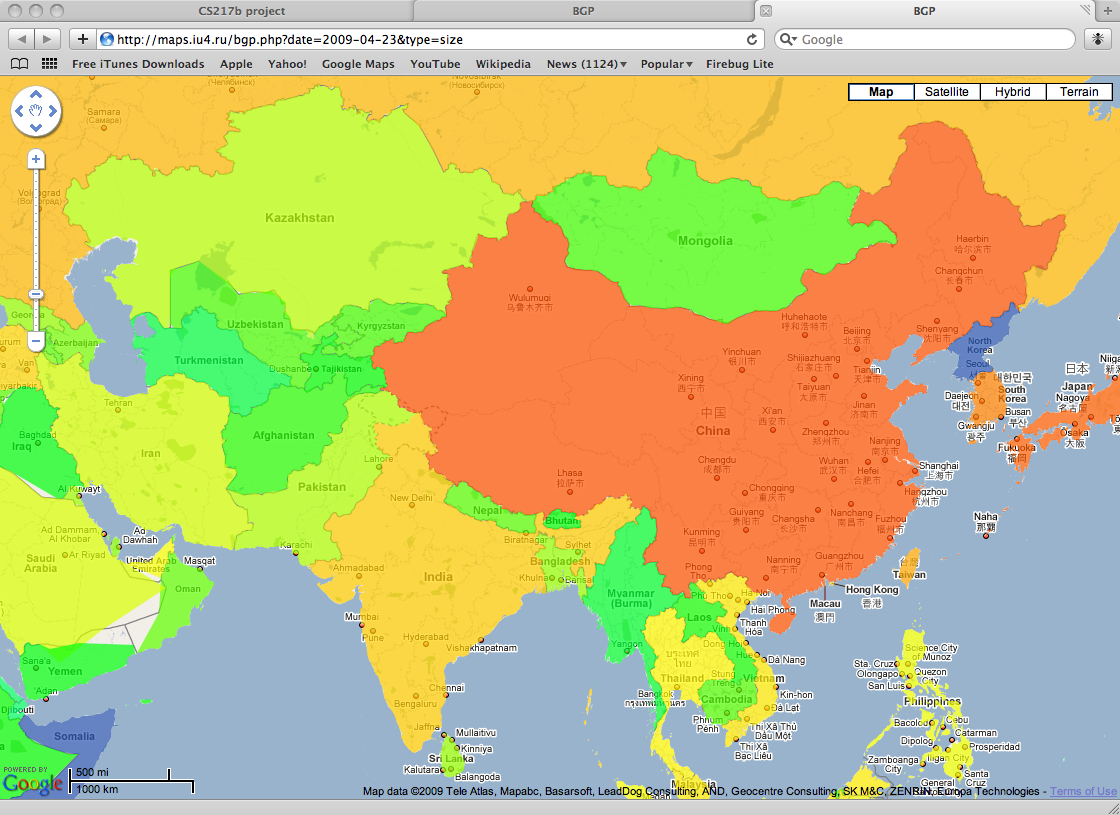
\includegraphics[trim=0 17px 0px 76px,clip=true,width=\columnwidth]{00_maps/asia_2009_space}%
		\hspace{-0.98\columnwidth}%
		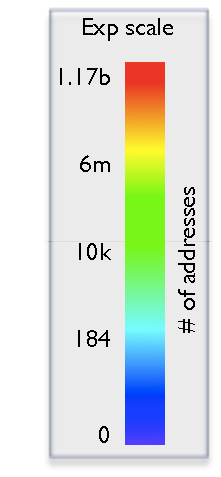
\includegraphics[width=1cm]{scale_bgp_size}\hspace{-1cm}%
		\hspace{0.98\columnwidth}
	\caption{Geographical distribution of announced IP space in Asian region on \textbf{April 23, 2009}}
	\label{fig:bgp ip space asia 2009}
% \end{figure}
\end{minipage}

\end{figure*}

\clearpage

\begin{table*}[p]
%%%%%%%%%%%%%%%%%%%%%%%%%%%%%%%%%%%%%%%%%%%%%%%%%%%%%%%%%%%%%%%%%%%%%%%%%%%%%%%%
%% TOP announced prefixes
%%%%%%%%%%%%%%%%%%%%%%%%%%%%%%%%%%%%%%%%%%%%%%%%%%%%%%%%%%%%%%%%%%%%%%%%%%%%%%%%
\begin{minipage}[t]{0.48\textwidth}
% \begin{table}[p]
	\begin{center}
	\caption{Top 25 countries with the most number of announced prefixes in BGP table on \textbf{January 1, 2003}}
	\label{tab:top25 bgp prefixes 2003}
	\begin{tabular}{|l||l|r|r|}
		\hline
		&      \bf Country		&    Prefixes   &       IP space 		\tabularnewline \hline 
1       &       US      		&       65849   &       759,792,816     \tabularnewline \hline
2       &       Unknown			&       6258    &       68,926,314      \tabularnewline \hline
3       &       Australia       &       5762    &       17,822,159      \tabularnewline \hline
4       &       Canada  		&       5612    &       38,912,924      \tabularnewline \hline
5       &       Japan   		&       2633    &       58,905,280      \tabularnewline \hline
6       &       South Korea     &       2441    &       27,334,687      \tabularnewline \hline
7       &       Germany			&       1934    &       46,556,556      \tabularnewline \hline
8       &       India  			&       1931    &       2,943,040       \tabularnewline \hline
9       &       UK     			&       1873    &       32,626,649      \tabularnewline \hline
10      &       China  			&       1615    &       28,522,130      \tabularnewline \hline
11      &       Argentina       &       1477    &       2,017,448       \tabularnewline \hline
12      &       Hong Kong       &       1261    &       5,621,473       \tabularnewline \hline
13      &       Sweden  		&       1198    &       11,280,533      \tabularnewline \hline
14      &       France  		&       1148    &       31,320,040      \tabularnewline \hline
15      &       Mexico  		&       1059    &       5,275,520       \tabularnewline \hline
16      &       Romania 		&       994     &       667,136 		\tabularnewline \hline
17      &       Russia  		&       972     &       5,911,712       \tabularnewline \hline
18      &       Chile   		&       834     &       2,098,161       \tabularnewline \hline
19      &       Indonesia       &       830     &       1,170,560       \tabularnewline \hline
20      &       Italy   		&       791     &       13,324,288      \tabularnewline \hline
21      &       Brazil  		&       760     &       11,580,416      \tabularnewline \hline
22      &       Taiwan  		&       708     &       13,448,168      \tabularnewline \hline
23      &       Netherlands     &       689     &       19,939,341      \tabularnewline \hline
24      &       European Union  &       687     &       2,707,383       \tabularnewline \hline
25      &       Finland 		&       630     &       7,307,018       \tabularnewline \hline
% 26      &       South Africa    &       618     &       5,762,180       \tabularnewline \hline
% 27      &       New Zealand     &       566     &       3,828,620       \tabularnewline \hline
% 28      &       Switzerland     &       560     &       7,937,424       \tabularnewline \hline
% 29      &       Thailand        &       559     &       1,877,060       \tabularnewline \hline
% 30      &       Spain   		&       511     &       8,921,568       \tabularnewline \hline
	\end{tabular}
	\end{center}
% \end{table}
\end{minipage}
%
\quad
%
\begin{minipage}[t]{0.48\textwidth}
% \begin{table}[p]
	\begin{center}
	\caption{Top 25 countries with the most number of announced prefixes in BGP table on \textbf{April 23, 2009}}
	\label{tab:top25 bgp prefixes 2009}
	\begin{tabular}{|l||l|r|r|r|}
		\hline
		&      \bf Country		& \bf Prefixes  &       \bf IP space 	& \bf Change$^{*}$ 	\tabularnewline \hline 
1       &       US      		&       115780  &       1,170,481,177   & 1.54			\tabularnewline \hline
2       &       South Korea     &       14308   &       84,553,300      & 3.09			\tabularnewline \hline
3       &       China  			&       13188   &       223,990,021     & 7.85			\tabularnewline \hline
4       &       Australia       &       11329   &       37,818,072      & 2.12			\tabularnewline \hline
5       &       India   		&       11022   &       17,575,040      & 5.97			\tabularnewline \hline
6       &       Russia  		&       8650    &       26,664,224      & 4.51			\tabularnewline \hline
7       &       Canada  		&       8328    &       57,471,348      & 1.48			\tabularnewline \hline
8       &       Romania 		&       5729    &       7,348,881       & 11.02			\tabularnewline \hline
9       &       UK      		&       5269    &       63,871,082      & 1.96			\tabularnewline \hline
10      &       European Union  &       4937    &       87,825,582      & 32.44			\tabularnewline \hline
11      &       Japan   		&       4674    &       173,789,965     & 2.95			\tabularnewline \hline
12      &       Brazil  		&       4643    &       40,429,504      & 3.49			\tabularnewline \hline
13      &       Argentina       &       4142    &       9,721,411       & 4.82			\tabularnewline \hline
14      &       Germany 		&       4035    &       84,904,642      & 1.82			\tabularnewline \hline
15      &       Mexico  		&       3648    &       19,583,832      & 3.71			\tabularnewline \hline
16      &       Indonesia       &       3562    &       5,248,256       & 4.48			\tabularnewline \hline
17      &       Hong Kong       &       3459    &       14,764,300      & 2.63			\tabularnewline \hline
18      &       Unknown   		&       3393    &       37,265,411      & 				\tabularnewline \hline
19      &       Bulgaria        &       3325    &       4,439,040       & 7.72			\tabularnewline \hline
20      &       Colombia        &       3029    &       4,901,340       & 11.86			\tabularnewline \hline
21      &       Ukraine 		&       3028    &       5,547,136       & 7.67			\tabularnewline \hline
22      &       Egypt  			&       2992    &       3,854,848       & 4.60			\tabularnewline \hline
23      &       France 			&       2511    &       61,070,996      & 1.95			\tabularnewline \hline
24      &       Taiwan 			&       2511    &       36,623,744      & 2.72			\tabularnewline \hline
25      &       Chile  			&       2375    &       6,101,376       & 2.91			\tabularnewline \hline
% 26      &       Poland 			&       2341    &       15,122,881      & 4.06			\tabularnewline \hline
% 27      &       Thailand        &       2039    &       7,210,800       & 3.84			\tabularnewline \hline
% 28      &       Spain   		&       1989    &       25,315,136      & 2.84			\tabularnewline \hline
% 29      &       Sweden  		&       1942    &       18,532,345      & 1.64			\tabularnewline \hline
% 30      &       Turkey  		&       1940    &       14,309,632      & 6.41			\tabularnewline \hline
	\end{tabular}
	\end{center}
	
	\small	$^{*}$ -- Relative change in number of prefixes in BGP announcements from January 1, 2003 and April 23, 2009
% \end{table}
\end{minipage}

\vspace{1cm}

%%%%%%%%%%%%%%%%%%%%%%%%%%%%%%%%%%%%%%%%%%%%%%%%%%%%%%%%%%%%%%%%%%%%%%%%%%%%%%%%
%% TOP announced IP space
%%%%%%%%%%%%%%%%%%%%%%%%%%%%%%%%%%%%%%%%%%%%%%%%%%%%%%%%%%%%%%%%%%%%%%%%%%%%%%%%
\begin{minipage}[t]{0.48\textwidth}
% \begin{table}[p]
	\begin{center}
	\caption{Top 25 countries with the most number of announced IP space in BGP table on \textbf{January 1, 2003}}
	\label{tab:top25 bgp ip space 2003}
	\begin{tabular}{|l||l|r|r|}
		\hline
		&      \bf Country		&    Prefixes   &       IP space 		\tabularnewline \hline 
1       &       US      		&       65849   &       759,792,816     \tabularnewline \hline
2       &       Unknown		   	&       6258    &       68,926,314      \tabularnewline \hline
3       &       Japan   		&       2633    &       58,905,280      \tabularnewline \hline
4       &       Germany 		&       1934    &       46,556,556      \tabularnewline \hline
5       &       Canada  		&       5612    &       38,912,924      \tabularnewline \hline
6       &       UK      		&       1873    &       32,626,649      \tabularnewline \hline
7       &       France  		&       1148    &       31,320,040      \tabularnewline \hline
8       &       China   		&       1615    &       28,522,130      \tabularnewline \hline
9       &       South Korea     &       2441    &       27,334,687      \tabularnewline \hline
10      &       Netherlands     &       689     &       19,939,341      \tabularnewline \hline
11      &       Australia       &       5762    &       17,822,159      \tabularnewline \hline
12      &       Taiwan  		&       708     &       13,448,168      \tabularnewline \hline
13      &       Italy   		&       791     &       13,324,288      \tabularnewline \hline
14      &       Brazil  		&       760     &       11,580,416      \tabularnewline \hline
15      &       Sweden  		&       1198    &       11,280,533      \tabularnewline \hline
16      &       Spain   		&       511     &       8,921,568       \tabularnewline \hline
17      &       Switzerland     &       560     &       7,937,424       \tabularnewline \hline
18      &       Norway  		&       262     &       7,591,936       \tabularnewline \hline
19      &       Finland 		&       630     &       7,307,018       \tabularnewline \hline
20      &       Russia  		&       972     &       5,911,712       \tabularnewline \hline
21      &       South Africa    &       618     &       5,762,180       \tabularnewline \hline
22      &       Hong Kong       &       1261    &       5,621,473       \tabularnewline \hline
23      &       Austria 		&       317     &       5,405,664       \tabularnewline \hline
24      &       Mexico  		&       1059    &       5,275,520       \tabularnewline \hline
25      &       Denmark 		&       196     &       4,169,984       \tabularnewline \hline
% 26      &       New Zealand     &       566     &       3,828,620       \tabularnewline \hline
% 27      &       Belgium 		&       175     &       3,796,224       \tabularnewline \hline
% 28      &       Poland  		&       273     &       3,721,216       \tabularnewline \hline
% 29      &       Malaysia        &       235     &       3,182,400       \tabularnewline \hline
% 30      &       India   		&       1931    &       2,943,040       \tabularnewline \hline
	\end{tabular}
	\end{center}
	\ \newline\ \newline
% \end{table}
\end{minipage}
%
\quad
%
\begin{minipage}[t]{0.48\textwidth}
% \begin{table}[p]
	\begin{center}
	\caption{Top 25 countries with the most number of announced IP space in BGP table on \textbf{April 23, 2009}}
	\label{tab:top25 bgp ip space 2009}
	\begin{tabular}{|l||l|r|r|r|}
		\hline
		&      \bf Country		& \bf Prefixes  &       \bf IP space 	& \bf Change$^{*}$ 	\tabularnewline \hline 
1       &       US      		&       115780  &       1,170,481,177   & 1.76			\tabularnewline \hline
2       &       China   		&       13188   &       223,990,021     & 8.17			\tabularnewline \hline
3       &       Japan   		&       4674    &       173,789,965     & 1.78			\tabularnewline \hline
4       &       European Union  &       4937    &       87,825,582      & 7.19			\tabularnewline \hline
5       &       Germany 		&       4035    &       84,904,642      & 2.09			\tabularnewline \hline
6       &       South Korea     &       14308   &       84,553,300      & 5.86			\tabularnewline \hline
7       &       UK      		&       5269    &       63,871,082      & 2.81			\tabularnewline \hline
8       &       France  		&       2511    &       61,070,996      & 2.19			\tabularnewline \hline
9       &       Canada  		&       8328    &       57,471,348      & 1.48			\tabularnewline \hline
10      &       Brazil  		&       4643    &       40,429,504      & 6.11			\tabularnewline \hline
11      &       Australia       &       11329   &       37,818,072      & 1.97			\tabularnewline \hline
12      &       Unknown			&       3393    &       37,265,411      & 				\tabularnewline \hline
13      &       Taiwan  		&       2511    &       36,623,744      & 3.55			\tabularnewline \hline
14      &       Italy   		&       1686    &       32,551,268      & 2.13			\tabularnewline \hline
15      &       Netherlands     &       1883    &       27,122,689      & 2.73			\tabularnewline \hline
16      &       Russia  		&       8650    &       26,664,224      & 8.90			\tabularnewline \hline
17      &       Spain   		&       1989    &       25,315,136      & 3.89			\tabularnewline \hline
18      &       Mexico  		&       3648    &       19,583,832      & 3.44			\tabularnewline \hline
19      &       Sweden  		&       1942    &       18,532,345      & 1.62			\tabularnewline \hline
20      &       India   		&       11022   &       17,575,040      & 5.71			\tabularnewline \hline
21      &       Poland  		&       2341    &       15,122,881      & 8.58			\tabularnewline \hline
22      &       Hong Kong       &       3459    &       14,764,300      & 2.74			\tabularnewline \hline
23      &       Turkey  		&       1940    &       14,309,632      & 8.40			\tabularnewline \hline
24      &       South Africa    &       1218    &       12,969,116      & 1.97			\tabularnewline \hline
25      &       Argentina       &       4142    &       9,721,411       & 2.80			\tabularnewline \hline
% 26      &       Vietnam        	&       1010    &       9,514,496       & 50.50			\tabularnewline \hline
% 27      &       Switzerland     &       1230    &       9,244,448       & 2.20			\tabularnewline \hline
% 28      &       Denmark 		&       569     &       9,239,192       & 2.90			\tabularnewline \hline
% 29      &       Malaysia        &       572     &       8,791,684       & 2.43			\tabularnewline \hline
% 30      &       Finland 		&       469     &       8,691,972       & 0.74			\tabularnewline \hline
	\end{tabular}
	\end{center}
	\small	$^{*}$ -- Relative change in globally announced IP space from January 1, 2003 and April 23, 2009
% \end{table}
\end{minipage}

\end{table*}

\clearpage


\subsection{BGP table growth accelerators}

\subsubsection{IP block fragmentation}
Third, we will build a graph showing both the approximated BGP table size and a calculated table size had there been no fragmenting of allocated blocks.

\begin{figure}[htbp]
	\centering
		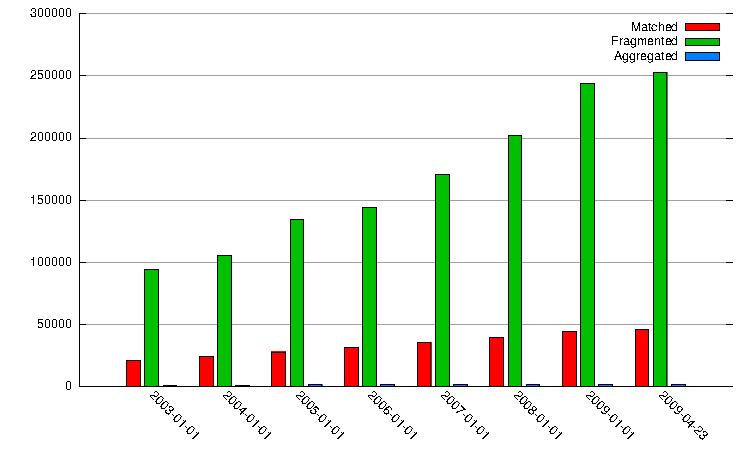
\includegraphics[width=\columnwidth]{05_matched_fragmented/frag-3}
	\caption{Dynamics of matched, fragmented, and aggregated IP prefixes in BGP announcements}
	\label{fig:fragmentation}
\end{figure}

\subsubsection{Duplicate announcements of IP blocks}
Fifth, we will determine the trends of the percentage of covering prefixes that 1) match, 2) fragment, and 3) aggregate allocations.
Sixth, we will show the dynamics of "Level 1" and "Level 2+" covered prefixes over time. Plus, we will give a comparison of covering prefixes to the number of allocations.  All these measurements concern the overall growth of the BGP routing table.

\begin{figure}[htbp]
	\centering
		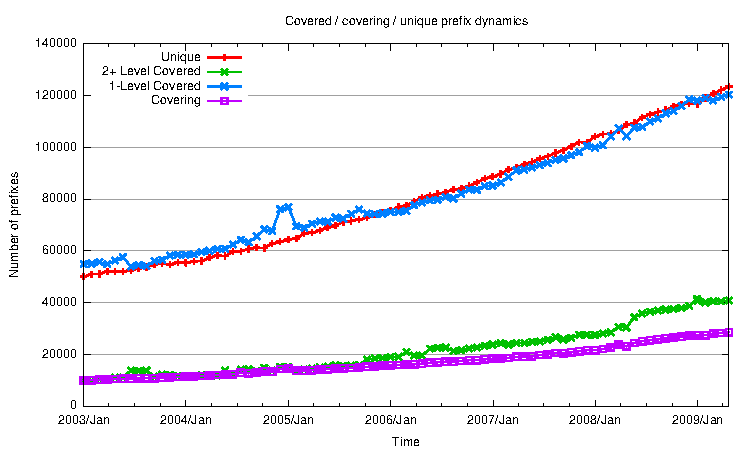
\includegraphics[width=\columnwidth]{06_covered/cover-3}
	\caption{Dynamics of covered, covering, and unique IP prefixes in BGP announcements}
	\label{fig:label}
\end{figure}
